%%%%%%%%%%%%%%%%%%%%%%%%%%%%%%%%%%%%%%%%%%%%%%%%%%%%%%%%%%%%%%%%%%%%%%
% main.tex
% Template de documento LaTeX para proyecto de fin de curso de Sistemas Embebidos para Tiempo Real
%
% Version 1.0 (IIE-FING-UDELAR)
% * Version inicial
%
%-- Leonardo Barboni, Julián Oreggioni
%    lbarboni@fing.edu.uy, juliano@fing.edu.uy
%
%%%%%%%%%%%%%%%%%%%%%%%%%%%%%%%%%%%%%%%%%%%%%%%%%%%%%%%%%%%%%%%%%%%%%%
% !TeX program = latexmk
% !BIB program = bibtex
\documentclass[a4paper,12pt]{article}

\usepackage{amsmath,amssymb}             
\usepackage{amsfonts}
\usepackage[utf8]{inputenc}   
\usepackage[spanish]{babel}
\selectlanguage{spanish} 
\usepackage[ruled,vlined,spanish]{algorithm2e}
\usepackage[T1]{fontenc}
\usepackage[left=2cm,right=2cm,top=1cm,bottom=1.5cm,includefoot,includehead,headheight=13.6pt]{geometry}
\usepackage{aecompl}
\usepackage[pdftex]{graphicx}
\graphicspath{{./figs/}}
\usepackage{color}
\usepackage{url}
\usepackage[font=small,labelfont=bf,tableposition=top]{caption}
\usepackage[most]{tcolorbox}
\usepackage{lineno}
\usepackage[numbers,sort&compress]{natbib}
\usepackage{listings}
\usepackage{fancyhdr, lastpage}
\usepackage{longtable}
\usepackage{afterpage}
\usepackage{textcomp}

\hyphenpenalty=13000

%----------------------                      
\pagestyle{fancy} 
\fancyhf{}                                             
\fancyfoot[C]{\hrule \bfseries\thepage}                   
\fancyhead[C]{\bfseries\nouppercase{Proyecto - Sistemas Embebidos Para Tiempo Real - 2025}}     

\fancypagestyle{firstpage}{
\pagestyle{fancy} 
\fancyhf{}                                             
\fancyfoot[C]{\hrule}                   
\fancyhead[C]{\bfseries\nouppercase{Proyecto - Sistemas Embebidos Para Tiempo Real - 2025}}     
}

%+++++++++++++++

\renewcommand{\contentsname}{Tabla de Contenido}
\renewcommand{\listtablename}{Índice de tablas}
\renewcommand{\tablename}{Tabla} 

%+++++++++++++++

\begin{document}

\thispagestyle{firstpage}

\begin{linenumbers} %COMENTAR PARA SACAR NUMERACION DE LINEAS

  \tcbset{
    frame code={},
    center title,
    left=0pt,
    right=0pt,
    top=0pt,
    bottom=0pt,
    colback=gray!70,
    colframe=white,
    width=\dimexpr\textwidth\relax,
    enlarge left by=0mm,
    boxsep=5pt,
    arc=0pt,outer arc=0pt,
  }



  \vspace{0.5in}
  \begin{tcolorbox}
    \centerline{\sc  \large \textbf {Especificaci\'on completa del Proyecto}}
    \vspace{2pc}
    \centerline{\sc \large \textbf {Alfombra de baile interactiva}}
    \vspace{1pc}
    \centerline{\sc \large \textbf {}}
    \vspace{1pc}
    \centerline{\sc \textbf {Autores:} Fabricio Correa, Ricardo Llorente, Gennaro Monetti }
    \vspace{2pc}
    \centerline{\textbf {Emails:} fabricio.correa@fing.edu.uy,ricardo.llorente@fing.edu.uy,}
    \centerline{\textbf gennaro.monetti@fing.edu.uy}
    \vspace{2pc}
    \end{tcolorbox}
    \centerline{\textbf {Tutores}: Josefina Lema}
    \vspace{1pc}
    \centerline{\textbf {Emails:} jlema@fing.edu.uy}
    \vspace{2pc}
    \centerline{Instituto de Ingenier\'ia El\'ectrica - Facultad de Ingenier\'ia - UDELAR}
    \vspace{2pc} 
    \noindent\rule{17cm}{0.4pt}
    \vspace{2pc}
        




  \tcbset{
    frame code={}
    center title,
    left=0pt,
    right=0pt,
    top=0pt,
    bottom=0pt,
    colback=gray!20,
    colframe=white,
    width=\dimexpr\textwidth\relax,
    enlarge left by=0mm,
    boxsep=5pt,
    arc=0pt,outer arc=0pt,
  }

  \begin{tcolorbox}
    \textsc{\textbf{Resumen}}\\
    \newline
    Resumir el proyecto en no mas de 200 palabras. Recordar que la documentaci\'on no debe superar las 25 carillas, sin incluir esta car\'atula ni la 
tabla de contenidos o anexos. Recuerde que el resumen es una descripci\'on corta, concreta y clara de los temas desarrollados, as\'i como tambi\'en de los m\'etodos y herramientas utilizados y de los resultados obtenidos. Agregar una muy breve descripci\'on de las conclusiones a las que se ha llegado.
    
  \end{tcolorbox}

  %+++++++++++++++++++++++

  \newpage
  \setcounter{page}{1}
  \tableofcontents

  %+++++++++++++++++++++++
  \section{previa}
  \label{sec:previa}

  Categoría 3: Alfombra de baile interactiva Tutor: Josefina Lema Cantidad de proyectos: hasta 3 Descripción El objetivo de esta categoría de proyectos es diseñar un sistema que emule una alfombra de baile interactiva, como la que se ve en la figura. Se deberá programar un sistema embebido capaz de detectar las interacciones del usuario y compararlos con una secuencia desplegada en una pantalla. En un primer lugar, se desarrollará una aplicación sencilla que muestre una secuencia de flechas en una pantalla OLED, indicando los pasos que el usuario debe seguir. 
La detección de los pasos se realizará mediante un teclado estándar matricial, registrando cuándo y que tecla fue seleccionada. Se debe llevar la cuenta del puntaje obtenido dependiendo de si el usuario presiona la tecla correcta en un rango de tiempo aceptable. 

El juego finaliza cuando se completa una secuencia de longitud fija o se pierde si el usuario se equivoca una determinada cantidad de veces. 



A este sistema se le pueden agregar diferentes variantes:
\begin{itemize}
    \item Variar el puntaje dependiendo de la precisión con la que se presiona: si el usuario presiona el botón correcto en el momento exacto se le asigna la mayor cantidad de puntos. Cuanto mayor sea el desfasaje de tiempo menor es la cantidad de puntos.
    \item Desarrollar distintas dificultades entre las cuales el usuario elige al iniciar el juego.
    \item Aumentar la dificultad durante una partida ya sea aumentando la velocidad o haciendo que la secuencia tenga más de una flecha a la vez.
\end{itemize}

El sistema consiste en:
\begin{itemize}
    \item Launchpad MSP-EXP430G2ET
    \item Display OLED SSD1306: se comunica con el microcontrolador utilizando comunicación I2C [1]. Se utilizará para desplegar las flechas de direcciones, así como las instrucciones de inicio y fin. El Proyecto [2,3] desarrolló un driver para el display OLED y una interfaz gráfica.
    \item Teclado matricial: se utiliza como interfaz de entrada para el usuario. Como alternativa se podrá utilizar el teclado de una PC mediante comunicación UART.
\end{itemize}

En años anteriores en el curso se implementaron otros juegos, ver por ejemplo Tetris controlado por UART [4,5] y Viborita [6].

Referencias 

[1] https://www.robotec.com.uy/productos/TX399 

[2] Heart Rate and Oxygen Saturation meter (HeroxS). Proyecto con manejo de display OLED. Proyecto de Sisem, 2022. 

[3] R D’eboli, J Schmitd, R Garcia Ordeig, J Oreggioni, HEROxS: Heart Rate and Oxygen Saturation Meter, Congreso Argentino de Sistemas Embebidos (CASE2023), Argentina, 10-11 ago, 2023 

[4] UARTetris: Tetris controlado por UART, Proyecto Sisem 2021 

[5] J. Pérez Mauri, J. Berniz, F. Morán, J. Oreggioni. U-Tetris: Tetris controlado por UART, Congreso Argentino de Sistemas Embebidos, CASE2021, Evento virtual, Argentina, 1-2 nov, 2021 

[6] Proyecto Sisem 2010 “Viborita” (CCuP)



\subsection{secciones a desarrollar}
\begin{itemize}
  \item Nombre del proyecto: corto y descriptivo
  \item Nombre de los integrantes y tutor
  \item Descripción del problema a ser resuelto: qué problema se va a abordar.
  \item Antecedentes: proyectos anteriores, artículos, libros, soluciones disponibles, etc.
  \item Objetivos del proyecto: qué se va a lograr, qué se va a entregar.
  \item Alcance del proyecto: definir claramente qué incluye y qué no.
  \item Descripción del sistema:
  \begin{itemize}
      \item Descripción funcional (lo que debe hacer)
      \item Diagrama de bloques (conceptual): división jerárquica/bloques constitutivos.
  \end{itemize}
  \item Requerimientos y restricciones del sistema:
  \begin{itemize}
      \item Procesamiento y memoria: estimación preliminar.
      \item Tiempos de respuesta: estimación de los tiempos de respuesta máximos requeridos.
  \end{itemize}
  \item Diseño preliminar:
  \begin{itemize}
      \item Plataforma de hardware: descripción de las partes, especificar si se necesita diseñar/construir hardware adicional y detallar qué.
      \item Arquitectura de software: describir la arquitectura justificando su selección.
  \end{itemize}
  \item Planificación:
  \begin{itemize}
      \item Actividades/tareas (nombre, descripción, duración)
      \item Describir las pruebas a realizar.
      \item Hito intermedio: describir entregables (buscar que coincidan con la fecha de la presentación)
      \item Cronograma.
  \end{itemize}
\end{itemize}


  \newpage
  \section{Descripción del problema}
  \label{sec:descripcion}
  La industria de los videojuegos y los sistemas interactivos ha tenido un crecimiento explosivo en las últimas décadas, abarcando no sólo consolas tradicionales, sino también dispositivos móviles, sistemas de realidad aumentada y plataformas físicas interactivas. Dentro de esta última categoría, destacan los juegos que combinan ejercicio físico y respuesta motora rápida, como las alfombras de baile interactivas. Uno de los casos más emblemáticos es el juego Dance Dance Revolution, lanzado en 1998 por Konami, que popularizó el uso de plataformas sensibles a la presión para seguir secuencias musicales en tiempo real.

  Estos sistemas, además de brindar entretenimiento, fomentan la actividad física y la coordinación motora, lo que los hace atractivos para públicos de todas las edades. A su vez, presentan desafíos interesantes desde el punto de vista de los sistemas embebidos: detección de eventos en tiempo real, evaluación de precisión temporal, control de interfaz gráfica, entre otros.

  Desde el punto de vista de esta propuesta, el problema a abordar consiste en diseñar un sistema embebido de bajo consumo que permita emular una alfombra de baile interactiva. El sistema deberá desplegar secuencias de flechas en una pantalla OLED y registrar las pulsaciones realizadas por el usuario en un teclado matricial. La evaluación del desempeño se realizará en base a la correspondencia y precisión temporal entre las pulsaciones y las flechas indicadas, otorgando puntajes y detectando condiciones de victoria o derrota.
  
  \section{Antecedentes}
  \label{sec:Antecedentes}
  
  Desde fines de los años 90, los videojuegos que combinan movimiento físico e interacción se volvieron muy populares. Entre ellos, el más representativo es Dance Dance Revolution (Konami, 1998) [1], que introdujo el concepto de alfombra sensible a la presión, donde el jugador debe seguir secuencias de flechas sincronizadas con música. Este tipo de juegos no solo son una forma de entretenimiento, sino que también fomentan la actividad física y la coordinación motriz.

  En el marco de la materia Sistemas Embebidos de Tiempo Real, se han desarrollado proyectos que sirven como referencia técnica para este trabajo. Entre ellos, el UARTetris \cite{Berniz2021}, que implementó el juego de Tetris utilizando comunicación UART y un display OLED controlado por un microcontrolador MSP430, y el proyecto Viborita \cite{Bellati2019}, donde se programó el clásico juego de la serpiente usando periféricos similares. Además, el proyecto Heart Rate and Oxygen Saturation Meter \cite{D’Eboli2022} utilizó pantallas OLED mediante comunicación I2C, incorporando la lectura y procesamiento de eventos en tiempo real.
  
  Estos antecedentes muestran que es posible, con los recursos disponibles (MSP430, pantalla OLED, teclado matricial), implementar un sistema embebido que maneje entradas de usuario en tiempo real, controle una interfaz gráfica y gestione puntajes o estados de juego.


  \section{Objetivos}
  \label{sec:Alcance}
  \subsection{Objetivo general}
  \label{sec:Objetivo general}
  Desarrollar un sistema embebido basado en el MSP430 que emule una alfombra de baile interactiva, capaz de detectar interacciones del usuario y compararlas con secuencias visuales en una pantalla OLED.
  \subsection{Objetivos específicos}
  \label{sec:Objetivos específicos}
  \begin{itemize}
    \item Programar toda la parte de codigo que gestione la entrada del usuario y la salida visual.
    \item Desarrollar una interfaz gráfica en una pantalla OLED que muestre secuencias de flechas y mensajes de estado.
    \item Implementar un teclado matricial como interfaz de entrada para el usuario, permitiendo registrar las pulsaciones.
    \item Evaluar el desempeño del usuario en función de la precisión temporal y la correspondencia con las secuencias mostradas.
    \item Definir condiciones de victoria y derrota, así como un sistema de puntajes basado en la precisión de las pulsaciones.
  \end{itemize}



  \section{Alcance}
  \label{sec:Alcance}

  El alcance del proyecto incluye el desarrollo de un sistema embebido que emule una alfombra de baile interactiva, utilizando un microcontrolador MSP430, una pantalla OLED y un teclado matricial. Se implementará la lógica del juego, la interfaz gráfica y la evaluación del desempeño del usuario. 

  El proyecto no incluirá el diseño o fabricación de hardware adicional, ni la integración con plataformas externas (alfombra física). Tampoco se abordarán aspectos relacionados con la conectividad inalámbrica o la compatibilidad con dispositivos distintos a los especificados.

  \section{Descripcion del sistema}
  \label{sec:Descripcion del sistema}
      \subsection{Descripción funcional}
      \label{sec:Descripción funcional} 
      El sistema debe ser capaz de realizar las siguientes funciones principales:

      \begin{itemize}
        \item Mostrar una secuencia de flechas en la pantalla OLED, indicando los pasos que el usuario debe seguir.
        \item Detectar las pulsaciones realizadas por el usuario en el teclado matricial.
        \item Evaluar si las pulsaciones coinciden con las flechas mostradas en pantalla y si se realizan dentro de un margen de tiempo permitido.
        \item Calcular y actualizar el puntaje del usuario en función de la precisión de las pulsaciones.
        \item Mostrar el puntaje actualizado en la pantalla OLED.
        \item Detectar condiciones de victoria (completar la secuencia correctamente) o derrota (cometer errores o exceder el tiempo permitido).
opcionales        
%        \item Permitir la selección de diferentes niveles de dificultad, ajustando la velocidad de las secuencias o la complejidad de las mismas.
%        \item Incrementar la dificultad durante el juego, como aumentar la velocidad o mostrar múltiples flechas simultáneamente.
        \item Finalizar la partida al completar la secuencia o al cometer errores.
      \end{itemize}
      \subsection{Diagrama de bloques}
      \label{sec:Diagrama de bloques}
      %%%%%%%%%%%%%%%%%%%%%%%%%%%%%%%
      %Agregar figura
      %%%%%%%%%%%%%%%%%%%%%%%%%%%%%%%
%      \begin{figure}[h]
%       \centering
%      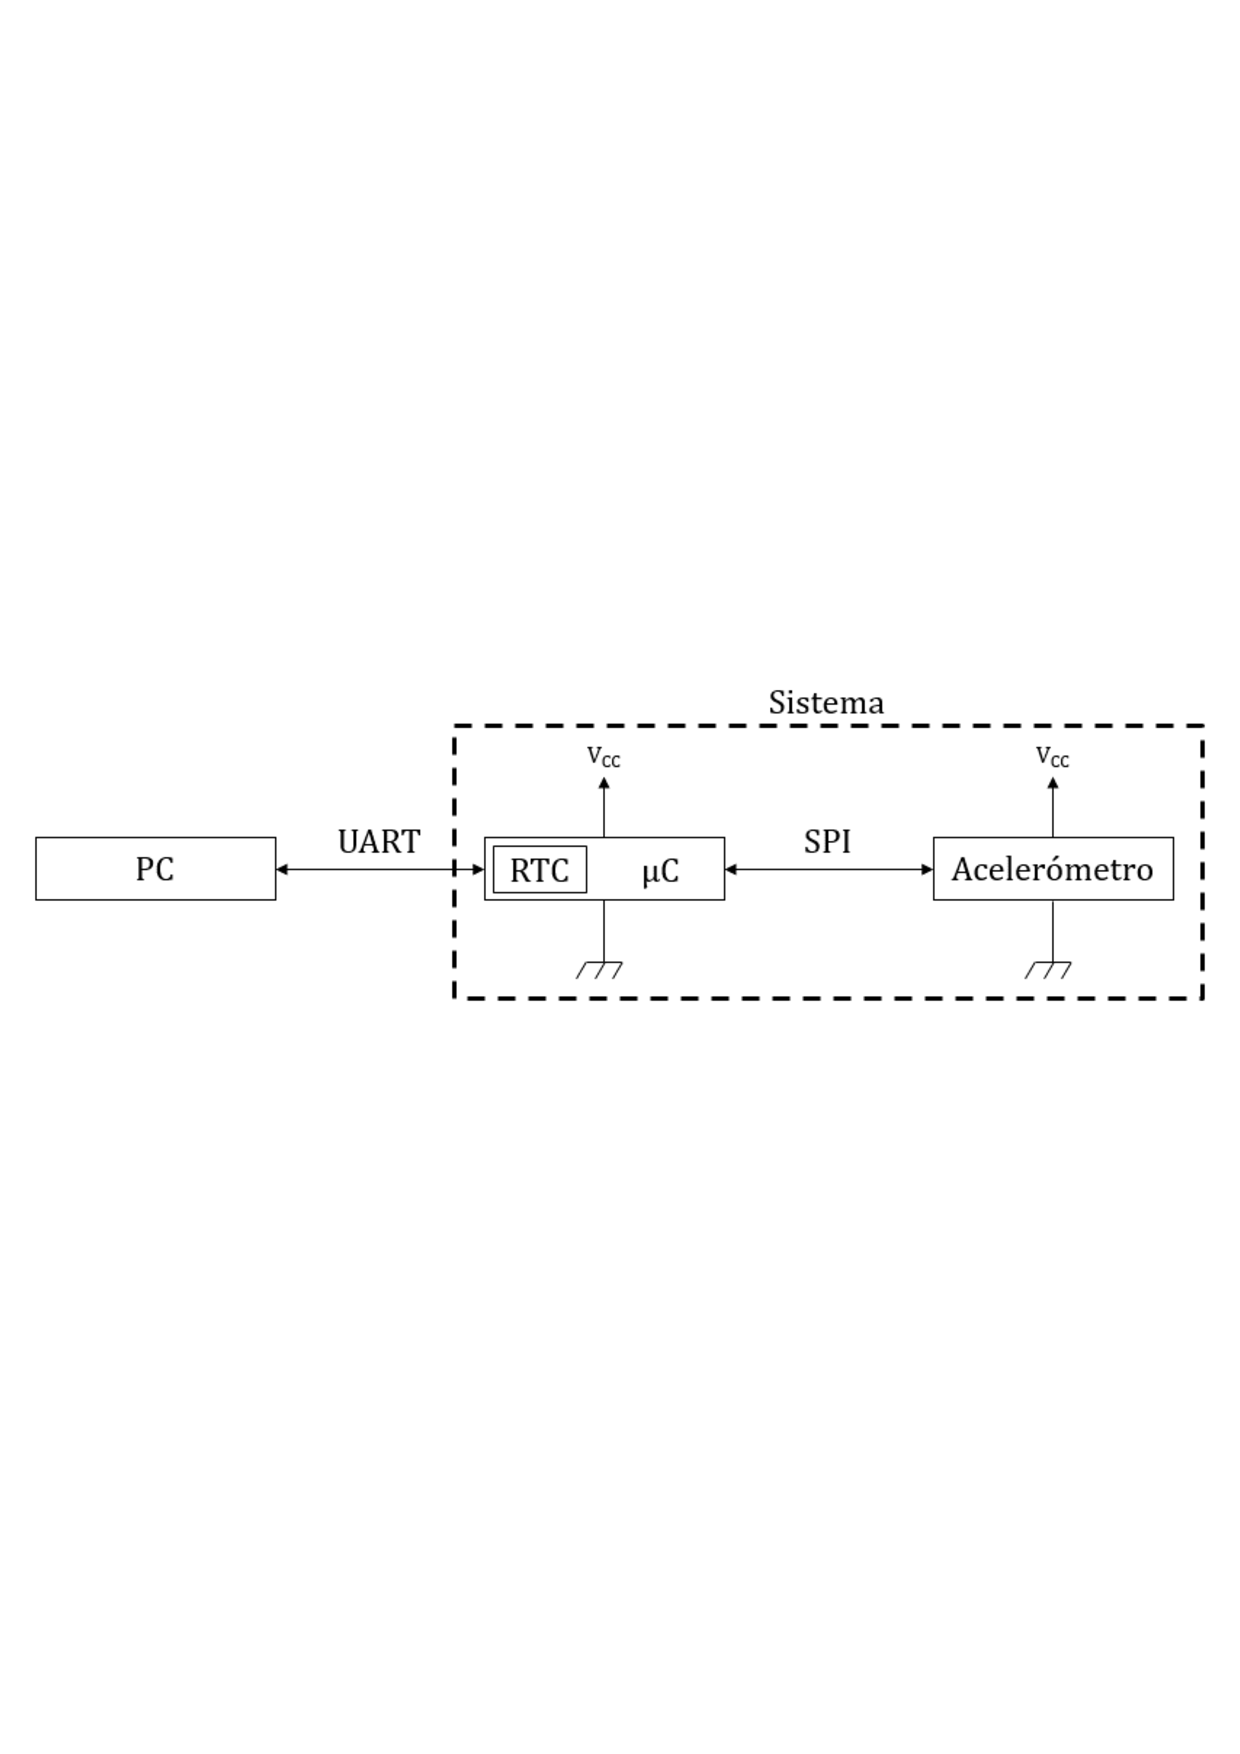
\includegraphics[width=0.8\textwidth]{figs/bloques.pdf}
%        \caption{Diagrama de bloques del sistema}
%        \label{fig:Diagrama de bloques}
%      \end{figure}
%       %%%%%%%%%%%%%%%%%%%%%%%%%%%%%%%      
      

      El diagrama de bloques muestra la arquitectura general del sistema. 
      El microcontrolador MSP430 se encarga de gestionar la entrada del usuario a través del teclado matricial y de controlar la salida visual en la pantalla OLED. La lógica del juego, incluyendo la evaluación de las pulsaciones y el cálculo del puntaje, se implementa en el software que corre en el microcontrolador. La comunicación entre los diferentes componentes se realiza mediante protocolos estándar (I2C para la pantalla OLED y GPIO para el teclado matricial).


  \section{Requerimientos y restricciones del sistema}
  \label{sec:Requ_Rest}
      \subsection{Procesamiento y memoria}
      \label{sec:Procesamiento y memoria}
      \begin{itemize}
        \item MSP430 tiene recursos limitados: se requiere gestión eficiente de memoria RAM y FLASH.
        \item Almacenamiento básico: secuencia actual, entrada del usuario, puntaje.
      \end{itemize} 


      \subsection{Tiempos de respuesta}
      \label{sec:Tiempos de respuesta}   
      \begin{itemize}
        \item Mostrar la siguiente flecha dentro de 100 ms después de una entrada correcta.
        \item Evaluar pulsaciones dentro de una ventana de 500 ms para considerar precisión "perfecta", más amplio para "aceptable".
        \item Mostrar el puntaje actualizado en la pantalla OLED en menos de 200 ms después de cada entrada.
        \item Cambiar la secuencia de flechas en menos de 200 ms después de completar una secuencia.
        \item Detectar condiciones de victoria o derrota en menos de 500 ms después de la última entrada del usuario.
        \item Responder a la entrada del usuario en menos de 100 ms después de una pulsación. 
        \item Almacenamiento básico: secuencia actual, entrada del usuario, puntaje.
      \end{itemize} 
  \section{Diseño preliminar}
  \label{sec:Diseño preliminar}
      \subsection{Plataforma de hardware}
      \label{sec:Plataforma de hardware}
      \begin{itemize}
        \item Microcontrolador: MSP430G2ET, con recursos limitados (memoria y procesamiento).
        \item Pantalla OLED SSD1306: comunicación I2C, para mostrar flechas e información.
        \item Teclado matricial: interfaz de entrada para el usuario.
      \end{itemize}
      \subsection{Arquitectura de software}
      \label{sec:Arquitectura de software}

  \section{Planificación}
  \label{sec:Planificación}
      \subsection{Actividades/tareas}
      \label{sec:Actividades}
      \subsection{Descripción de las pruebas a realizar}
      \label{sec:Descripción de las pruebas a realizar}
      \subsection{Hito intermedio}
      \label{sec:Hito intermedio}
      \subsection{Cronograma}
      \label{sec:Cronograma}
 

  \newpage
  



  


  

  
  %++++++++++++++++++++++++++++++++++++
  \addcontentsline{toc}{section}{Bibliograf\'ia}
  \renewcommand{\refname}{Bibliograf\'ia}
  \bibliographystyle{IEEEtran}
  \bibliography{refs}



\end{linenumbers} %COMENTAR PARA SACAR NUMERACION DE LINEAS


\end{document}
